\documentclass[12pt]{exam}
\usepackage{amsthm}
\usepackage{libertine}
\usepackage[utf8]{inputenc}
\usepackage[margin=1in]{geometry}
\usepackage{amsmath,amssymb}
\usepackage{multicol}
\usepackage[shortlabels]{enumitem}
\usepackage{siunitx}
\usepackage{cancel}
\usepackage{graphicx}
\usepackage{pgfplots}
\usepackage{listings}
\usepackage{tikz}


\pgfplotsset{width=10cm,compat=1.9}
\usepgfplotslibrary{external}
\tikzexternalize

\newcommand{\class}{Física Moderna - Complementaria} % This is the name of the course 
\newcommand{\examnum}{Trabajo 6} % This is the name of the assignment
\newcommand{\examdate}{03/03/2023} % This is the due date
\newcommand{\timelimit}{}





\begin{document}
\pagestyle{plain}
\thispagestyle{empty}

\noindent
\begin{tabular*}{\textwidth}{l @{\extracolsep{\fill}} r @{\extracolsep{6pt}} l}
\textbf{\class} & \textbf{Name:} & \textit{David Santiago Pachon Ballen}\\ %Your name here instead, obviously 
	\textbf{\examnum} &&\textit{Sergio Montoya Ramírez}\\
\textbf{\examdate} &&\\
\end{tabular*}\\
\rule[2ex]{\textwidth}{2pt}
% ---




\begin{enumerate} %You can make lists!
	\item \begin{enumerate}
			\item $A$
				Para encontrar A despejemos desde la integral
				\begin{align*}
					&\int_{-\infty}^\infty \psi^2 dx = 1\\
					&\int_{-\infty}^\infty A^2e^{-\frac{2x^2}{a_0^2}}=1\\
					&A^2\int_{-\infty}^\infty e^{-\frac{2x^2}{a_0^2}}dx\\
					&\int_{-\infty}^{\infty} e^{-bx^2}dx = \sqrt{\frac{\pi}{b}}\text{ Gaussiana }\\
					&b = \frac{2}{a_0^2}\\
					&A^2\sqrt{\frac{\pi a_0^2}{2}} = 1\\
					&A^2 = \sqrt{\frac{2}{\pi a_0^2}}\\
					&A = \sqrt[4]{\frac{2}{\pi a_0^2}}
				\end{align*}
			\item \begin{align*}
					&<p> = \int_{-\infty}^{\infty}\psi* \frac{\hbar}{i}\frac{\partial\phi}{\partial x}dx\\
					&\frac{\partial \psi}{\partial x} = \frac{-2x}{a_0^2}Ae^{-\frac{x^2}{a_0^2}}\\
					& = \frac{\hbar}{i}\int_{-\infty}^{\infty}xA^2e^{-\frac{2x^2}{a_0^2}}dx\\
					& = 0
			\end{align*}
			Nota que la función que esta adentro es una función impar y como el intervalo en el que estamos integrando es par entonces esta integral es 0
			\item Para este caso necesitaremos definir $\hat{p}^2 = \hbar \frac{\partial^2}{\partial x^2}$ en particular necesitaremos hallarlo aplicado en $\psi$ por lo tanto esto nos quedaria
				\begin{align*}
					&<p^2> = \int_{-\infty}^{\infty} \hbar \psi \frac{\partial^2 \psi}{\partial x^2}\\
					&\frac{\partial^2 \psi}{\partial x^2} = \frac{2Ae^{-\frac{x^2}{a_0^2}}(a_0^2-2x^2)}{a_0^4} \text{ Sacado de Wolfram }\\
					&= \psi \cdot \frac{\partial^2 \psi}{\partial x^2} = Ae^{-\frac{x^2}{a_0^2}}\cdot \frac{2Ae^{-\frac{x^2}{a_0^2}}(a_0^2-2x^2)}{a_0^4}\\
					&= \frac{A^2e^{-\frac{2x^2}{a_0^2}}(a_o^2-2x^2)}{a_0^4}\\
					&=\frac{\hbar A^2}{a_0^4} \int_{-\infty}^{\infty}e^{-\frac{2x^2}{a_0^2}}(a_0^2 -2x^2)\\
					&=\frac{\hbar A^2}{a_0^4} \left(\int_{-\infty}^{\infty}a_0^2e^{-\frac{2x^2}{a_0}} - \int_{-\infty}^{\infty}2x^2e^{-\frac{2x^2}{a_0^2}}\right)\\
					&=\frac{\hbar A^2}{a_0^4} \left(a_0^2\sqrt{\frac{\pi a_0^2}{2}}-\frac{1}{2}\sqrt{\frac{\pi}{2}}a_0^3\right)
				\end{align*}
			\item \begin{align*}
					&<x> = \int_{-\infty}^{\infty} Ae^{-\frac{x^2}{a_0^2}}x dx\\
					&<x> = 0
			\end{align*}
			Note que tal cual como en la sección (b), la función a integrar es impar y el intervalo par. Por lo tanto el valor es 0.
		\item \begin{align*}
				& <x^2> = \int_{-\infty}^{\infty}\psi*x^2\psi dx\\
				&=\int_{-\infty}^{\infty} Ae^{-\frac{x^2}{a_0^2}}x^2 Ae^{-\frac{x^2}{a_0^2}}dx\\
				&=A^2\int_{-\infty}^{\infty} x^2 e^{-\frac{2x^2}{a_0^2}}=A^2\frac{1}{4}\sqrt{\frac{\pi}{2}}a_0^3
		\end{align*}
	\item Ahora bien, para encontrar esto vamos a utilizar que
		\begin{align*}
			&\sigma_p = \sqrt{<p^2>-<p>^2}\\
			&\sigma_x = \sqrt{<x^2>-<x>^2}
		\end{align*}
			Con esto ya en mente notemos que $<x>$ y $<p>$ son 0 y por tanto su cuadrado tambien lo es lo que nos deja con unicamente
			\begin{align*}
				&\sigma_p = \sqrt{<p^2>}\\
				&\sigma_p = \sqrt{\frac{\hbar A^2}{a_0^4} \left(a_0^2\sqrt{\frac{\pi a_0^2}{2}}-\frac{1}{2}\sqrt{\frac{\pi}{2}}a_0^3\right)}\\
				&\sigma_x = \sqrt{<x^2>}\\
				&\sigma_x = \sqrt{A^2\frac{1}{4}\sqrt{\frac{\pi}{2}}a_0^3}
			\end{align*}
			Ahora una vez tenemos esto las multiplicamos que nos quedaria
			\begin{align*}
				&\sigma_p\sigma_x = \sqrt{\frac{\hbar A^2}{a_0^4} \left(a_0^2\sqrt{\frac{\pi a_0^2}{2}}-\frac{1}{2}\sqrt{\frac{\pi}{2}}a_0^3\right)A^2\frac{1}{4}\sqrt{\frac{\pi}{2}}a_0^3}\\
				&=\frac{A^2}{2a_0^2}\sqrt{\hbar \left(a_0^2\sqrt{\frac{\pi a_0^2}{2}}-\frac{1}{2}\sqrt{\frac{\pi}{2}}a_0^3\right)\sqrt{\frac{\pi}{2}}a_0^3}\\
				&=\frac{A^2}{2a_0^2}\sqrt{\hbar \left(\frac{\pi a_0^7}{2}-\frac{\pi}{4}a_0^6\right)}\\
				&=\frac{A^2a_0}{2}\sqrt{\hbar \left(\frac{\pi}{2}a_0-\frac{\pi}{4}\right)}
			\end{align*}
	\end{enumerate}
\item \begin{enumerate}
\item Para este caso vamos a dividir la derivada en intervalos en particular los intervalos que estan en de $0$ a $\frac{L}{2}$ y de $\frac{L}{2}$ a $L$. Los otros dos intervalos los ignoraremos pues como estamos en un pozo infinito lo que se sale de este caso podemos suponer que es 0. Esto nos deja con
	\begin{align*}
		&\int_{-\infty}^{\infty} \psi^2 dx = 1\\
		&\int_{0}^{\frac{L}{2}} A^2x^2 dx + \int_{\frac{L}{2}}^L (AL-Ax)^2 dx\\
		&\frac{A^2L^3}{12} = 1 \text{ Resultado sacado de Symbolab }\\
		&A = \sqrt{\frac{12}{L^3}}
	\end{align*}
	Esta es una expresión para una longitud general. Sin embargo, es imposible graficar con una longitud de este estilo. entonces determinamos que L=1 de manera arbitraria solo para que nuestra grafica tenga sentido. Esta grafica es la \ref{fig:Graf}
	\begin{figure}[h]
		\centering
		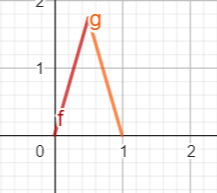
\includegraphics[scale=0.9]{Graf.jpeg}
		\caption{Grafica de la función hallada para una longitud aribtraria. En particular, L=1}
		\label{fig:Graf}
	\end{figure}

\item Para calcular la probabilidad que necesitamos vamos a utilizar 2 ecuaciones.
	\begin{align}
		&a_1 = \int_{-\infty}^{\infty}\sqrt{\frac{2}{L}}\psi(x)dx\\
		&P(E_1) = a_1^2
	\end{align}
	Ahora bien con esto podemos separa la división en los mismos intervalos que previamente lo que nos dejara con
		\begin{align*}
			&\sqrt{\frac{2}{L}}\left(\int_0^{\frac{L}{2}}Ax dx + \int_{\frac{L}{2}}^L (AL - Ax)dx\right)\\
			&\sqrt{\frac{2}{L}}\left(A\frac{L^2}{4} + AL - A\frac{3L^2}{4}\right)\\
			&a_i = \sqrt{\frac{2}{L}}\left(A\frac{L^2}{4} + AL - A\frac{3L^2}{4}\right)\\
			&P(E_1) = \frac{2}{L}\left(\frac{L^2}{2}+AL\right)^2
		\end{align*}
\end{enumerate}
\end{enumerate}

\end{document}
